\documentclass[12pt]{article}
\usepackage[margin=2.5cm]{geometry}
\usepackage{enumerate}
\usepackage{amsfonts}
\usepackage{amsmath}
\usepackage{fancyhdr}
\usepackage{amsmath}
\usepackage{amssymb}
\usepackage{amsthm}
\usepackage{mdframed}
\usepackage{graphicx}
\usepackage{subcaption}
\usepackage{adjustbox}
\usepackage{listings}
\usepackage{xcolor}
\usepackage{booktabs}
\usepackage[utf]{kotex}
\usepackage{hyperref}

\definecolor{codegreen}{rgb}{0,0.6,0}
\definecolor{codegray}{rgb}{0.5,0.5,0.5}
\definecolor{codepurple}{rgb}{0.58,0,0.82}
\definecolor{backcolour}{rgb}{0.95,0.95,0.92}

\lstdefinestyle{mystyle}{
    backgroundcolor=\color{backcolour},
    commentstyle=\color{codegreen},
    keywordstyle=\color{magenta},
    numberstyle=\tiny\color{codegray},
    stringstyle=\color{codepurple},
    basicstyle=\ttfamily\footnotesize,
    breakatwhitespace=false,
    breaklines=true,
    captionpos=b,
    keepspaces=true,
    numbers=left,
    numbersep=5pt,
    showspaces=false,
    showstringspaces=false,
    showtabs=false,
    tabsize=1
}

\lstset{style=mystyle}

\pagestyle{fancy}
\renewcommand{\headrulewidth}{0.4pt}
\lhead{CSC 209}
\rhead{Review 5 Solution}

\begin{document}
\title{CSC 209 Review 5 Solution}
\maketitle

\bigskip

\begin{enumerate}[1)]
    \item

    \bigskip

    \begin{enumerate}[a)]
        \item 14
        \item 34
        \item 4
        \item true
        \item false
    \end{enumerate}

    \underline{\textbf{Notes}}

    \begin{itemize}
        \item \textbf{Pointer Arithematic}

        \begin{itemize}
            \item Adding an integer to a pointer

            \bigskip

            \underline{\textbf{Example}}

            \begin{center}
            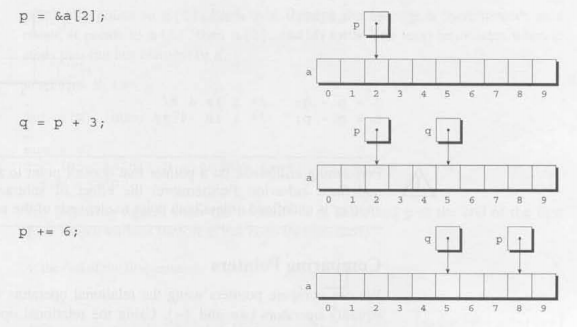
\includegraphics[width=\linewidth]{images/review_5_solution_1.png}
            \end{center}

            \bigskip

            \item Subtracting an integer from a pointer

            \bigskip

            \underline{\textbf{Example}}

            \begin{center}
            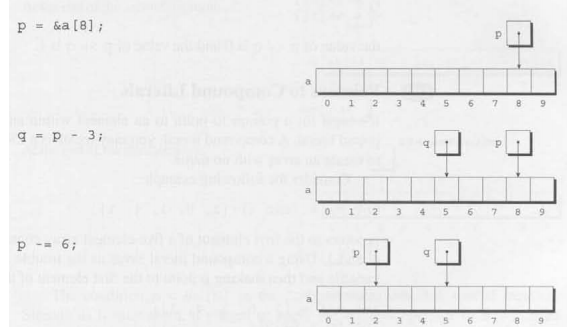
\includegraphics[width=\linewidth]{images/review_5_solution_2.png}
            \end{center}

            \bigskip

            \item Subtracting one pointer from another

            \bigskip

            \underline{\textbf{Example}}

            \begin{center}
            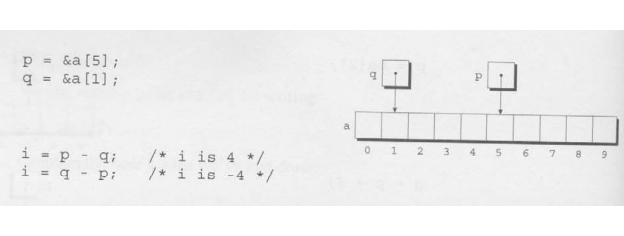
\includegraphics[width=\linewidth]{images/review_5_solution_3.png}
            \end{center}

        \end{itemize}

        \item \textbf{Comparing pointers}

        \begin{itemize}
            \item Can compare pointers using relational operators (i.e. $<,<=,>,>=$) and the equality operators (i.e. $==, !=$)
            \item Returns 1 if \texttt{true} and 0 if \texttt{false}

            \bigskip

            \underline{\textbf{Example}}

            \bigskip

            \texttt{p = \&a[5];}

            \texttt{q = \&a[1];}

            \bigskip

            \texttt{p $<=$ q} is 0 and \texttt{p $>=$ q} is 1


        \end{itemize}


    \end{itemize}
\end{enumerate}

\end{document}